\documentclass[a4paper, 12pt]{article}

\usepackage[T2A]{fontenc}    
\usepackage[utf8]{inputenc}
\usepackage[english,russian]{babel} 
\usepackage{amsmath}
\usepackage{graphicx}
\usepackage{float}
\renewcommand{\phi}{\varphi}

\begin{document}
Имеем два пучка света, один референтный
\[E_1 = E_0 \cos\omega t,\]
и один модулируемый
\[E_2 = E_0 \cos(\omega t + \phi(t)),\]

Референтный пучок проходит через золотую пленку и интерферирует с отраженным от нее модулируемым пучком.

Прошедший референтный пучок:
\[E_1^T = \tilde T E_0 \cos\omega t,\]

Отраженный модулируемый пучок:
\[E_2^R = \tilde R E_0 \cos(\omega t + \phi(t) + \pi).\]

\section{Простейший случай}
Рассмотрим случай, когда $\tilde T = T = const$, $\tilde R = R = const$ и $\phi(t) = \phi = const$.

\[I = \langle (E_1^T + E_2^R)^2 \rangle = \frac{E_0^2}{2} \left( T^2 + R^2 - 2 T R \cos\phi \right) = \bar{I} (T^2 + R^2 - 2 T R \cos\phi).\]

\begin{figure}[H]
  \centering
  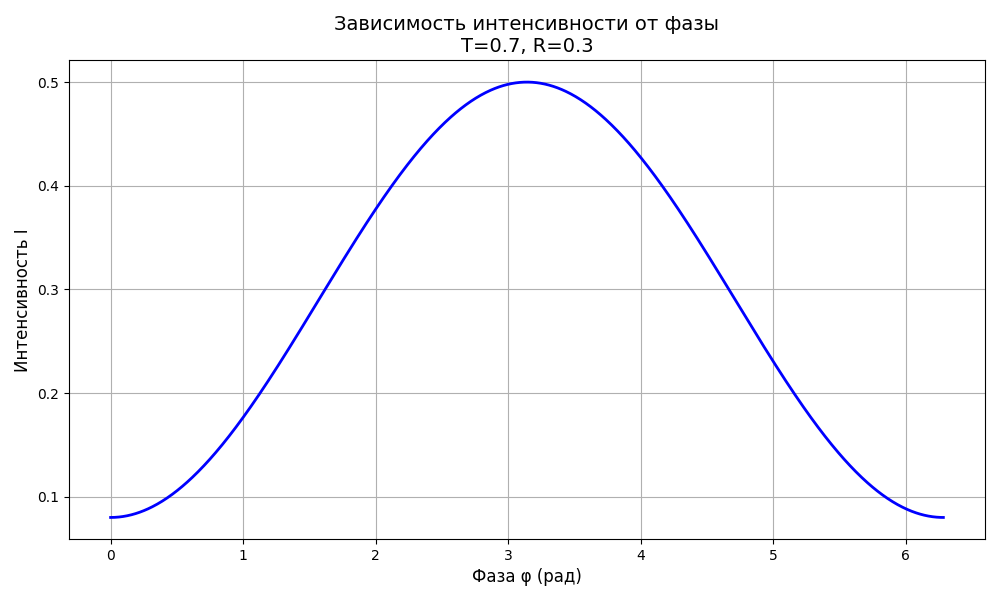
\includegraphics[width=0.5\textwidth]{../figures/intensity_vs_phase_T0.7_R0.3.png}
  \caption{Зависимость интенсивности от фазы в простейшем случае}
\end{figure}

\section{Случай гармонической модуляции}
Пусть снова $\tilde T = T = const$, $\tilde R = R = const$, но
\[\phi(t) = \phi_0 + \Phi \cos(\Omega t).\]

\[I(t) = \langle (E_1^T + E_2^R)^2 \rangle = \bar{I} \left( T^2 + R^2 - 2 T R \cos(\phi_0 + \Phi \cos(\Omega t)) \right).\]

Исходное выражение:

\[
  T^2 + R^2 - 2 T R \cos\left(\phi_0 + \Phi \cos(\Omega t)\right)
\]

Разложение в ряд Фурье по гармоникам \(\Omega\):

1. Постоянная составляющая:
\[
  I_0 = \bar{I} (T^2 + R^2 - 2 T R \cos\phi_0)
\]

2. Гармоники с частотами \(n\Omega\):
\[
  I_n = \bar{I} a_n \cos(n\Omega t),
\]
где коэффициенты \(a_n\) определяются следующим образом:
\begin{itemize}
  \item Для чётных \(n = 2k\) (\(k \geq 1\)):
        \[
          a_{2k} = -4 T R \cos\phi_0 \, (-1)^k J_{2k}(\Phi)
        \]
  \item Для нечётных \(n = 2k+1\) (\(k \geq 0\)):
        \[
          a_{2k+1} = 4 T R \sin\phi_0 \, (-1)^k J_{2k+1}(\Phi)
        \]
\end{itemize}

Первая гармоника:
\[
  I_1(t) = \bar{I} \left(a_1 \cos(\Omega t) + b_1 \sin(\Omega t)\right) = 4\bar{I}TR \sin\phi_0 \, J_1(\Phi) \cos(\Omega t)
\]

\begin{figure}[H]
  \centering
  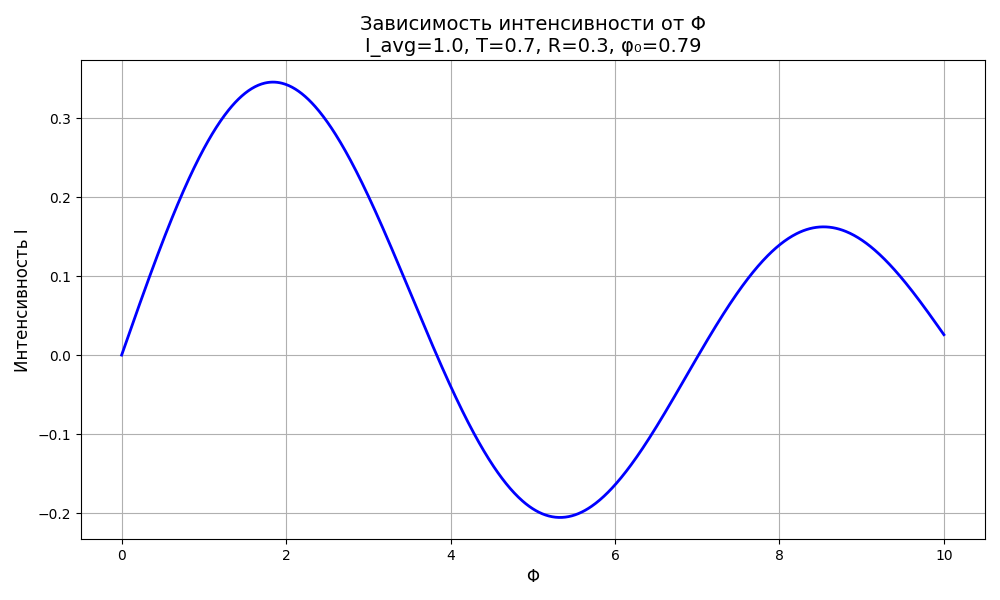
\includegraphics[width=0.5\textwidth]{../figures/bessel_intensity_I1.0_T0.7_R0.3_phi0.79.png}
  \caption{Первая гармоника}
\end{figure}

Вторая гармоника:
\[
  I_2(t) = \bar{I} \left(a_2 \cos(2\Omega t) + b_2 \sin(2\Omega t)\right) = 4\bar{I}TR \cos\phi_0 \, J_2(\Phi) \cos(2\Omega t).
\]

\begin{figure}[H]
  \centering
  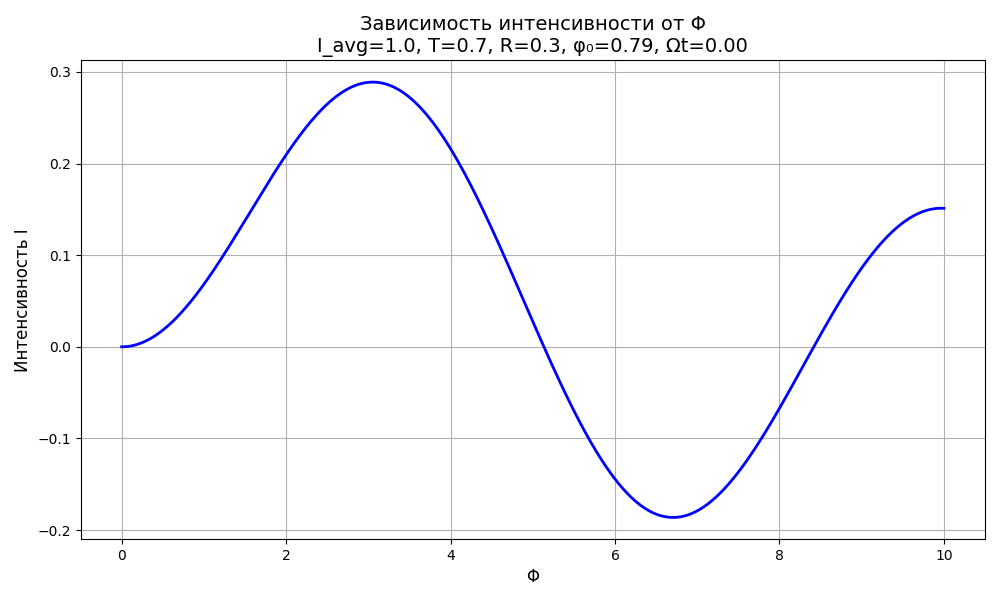
\includegraphics[width=0.5\textwidth]{../figures/bessel2_intensity_I1.0_T0.7_R0.3_phi0.79_Omega0.00.png}
  \caption{Вторая гармоника}
  \label{fig:bessel2_intensity_I1.0_T0.7_R0.3_phi0.00_Omega0.00}
\end{figure}

\section{Случай когерентного контроля}

Теперь $\tilde T = T_0 + T\cos(W\phi)$, $\tilde R = R_0 + R\cos(W\phi)$, $\phi(t) = \phi_0 + \Phi\cos(\Omega t)$.

\[ I = \langle (E_1^T + E_2^R)^2 \rangle = \bar I (\tilde{T}^2 + \tilde{R}^2) - 2 \bar I \tilde{T}\tilde{R} \cos\phi(t)\]

Для разложения усреднённого выражения \(\langle (E_1^T + E_2^R)^2 \rangle\) в ряд Фурье по гармоникам \(\Omega\) используем разложение Якоби-Ангера для функций с фазовой модуляцией \(\phi(t) = \phi_0 + \Phi \cos(\Omega t)\). Окончательный ряд Фурье имеет вид:

\begin{multline*}
  \langle (E_1^T + E_2^R)^2 \rangle = \sum_{n=-\infty}^{\infty} \left[ \bar I \left( T_0^2 + R_0^2 + \frac{T^2 + R^2}{2} \right) J_0(W\Phi) \delta_{n,0} \right] +\\+ \sum_{n \neq 0} \left[ A_n \cos(n\Omega t) + B_n \sin(n\Omega t) \right]
\end{multline*}

где коэффициенты \(A_n\) и \(B_n\) выражаются через функции Бесселя \(J_n\):

\[
  A_n = 2\bar I \left[ (T_0 T + R_0 R) J_n(W\Phi) \cos\left(W\phi_0 + \frac{n\pi}{2}\right) - T_0 R_0 J_n(\Phi) \cos\left(\phi_0 + \frac{n\pi}{2}\right) \right],
\]
\[
  B_n = 2\bar I \left[ (T_0 T + R_0 R) J_n(W\Phi) \sin\left(W\phi_0 + \frac{n\pi}{2}\right) - T_0 R_0 J_n(\Phi) \sin\left(\phi_0 + \frac{n\pi}{2}\right) \right].
\]

Первая гармоника:
\[
  I_1(t) = C_1 \cos\left(\Omega t + \theta_1\right),
\]
где:
\[
  \mathcal{A} = (T_0 T + R_0 R) J_1(W\Phi), \quad \mathcal{B} = T_0 R_0 J_1(\Phi).
\]
\[
  C_1 = 2\bar I \sqrt{
    \mathcal{A}^2 + \mathcal{B}^2 - 2 \mathcal{A} \mathcal{B} \cos\left((W-1)\phi_0\right)
  }.
\]
\[
  \theta_1 = \arctan\left(
  \frac{\mathcal{A} \cos(W\phi_0) - \mathcal{B} \cos\phi_0}
  {\mathcal{A} \sin(W\phi_0) - \mathcal{B} \sin\phi_0}
  \right).
\]

\begin{figure}[H]
  \centering
  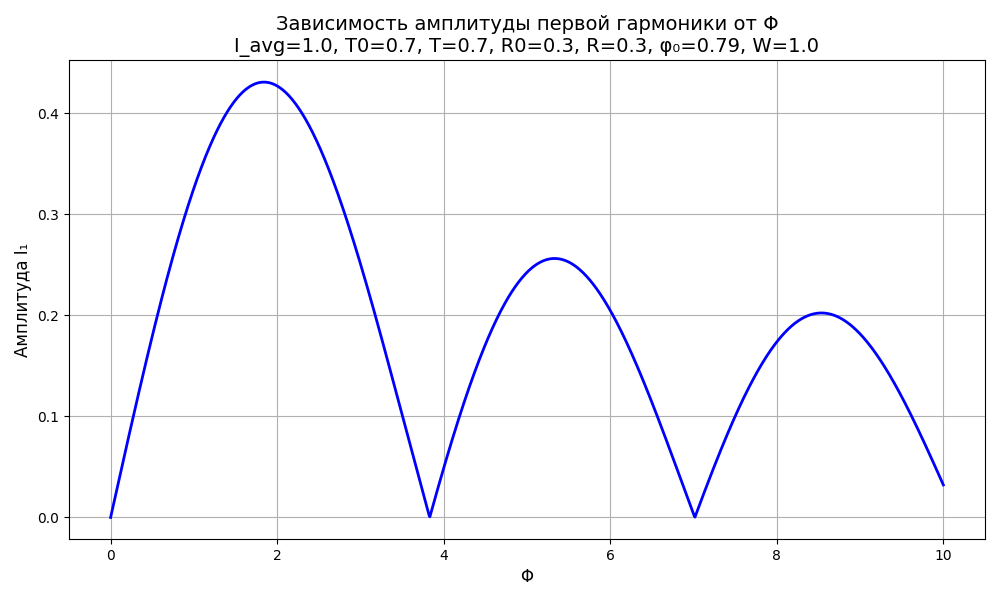
\includegraphics[width=0.5\textwidth]{../figures/first_harmonic_intensity_I1.0_T00.7_T0.7_R00.3_R0.3_phi0.79_W1.0.png}
  \caption{Первая гармоника}
\end{figure}

Вторая гармоника:
\[
  I_2(t) = C_2 \cos(2\Omega t + \theta_2),
\]
где:
\[
  C_2 = 2\bar I \sqrt{
    \mathcal{A}_2^2 + \mathcal{B}_2^2 - 2 \mathcal{A}_2 \mathcal{B}_2 \cos\left((2W-2)\phi_0\right)
  },
\]
\[
\theta_2 = \arctan\left(
\frac{\mathcal{A}_2 \cos(2W\phi_0) - \mathcal{B}_2 \cos(2\phi_0)}{\mathcal{A}_2 \sin(2W\phi_0) - \mathcal{B}_2 \sin(2\phi_0)}
\right),
\]
с коэффициентами:
\[
\mathcal{A}_2 = \frac{(T_0 T + R_0 R) J_2(W\Phi)}{2}, \quad \mathcal{B}_2 = \frac{T_0 R_0 J_2(\Phi)}{2}.
\]

\begin{figure}[H]
  \centering
  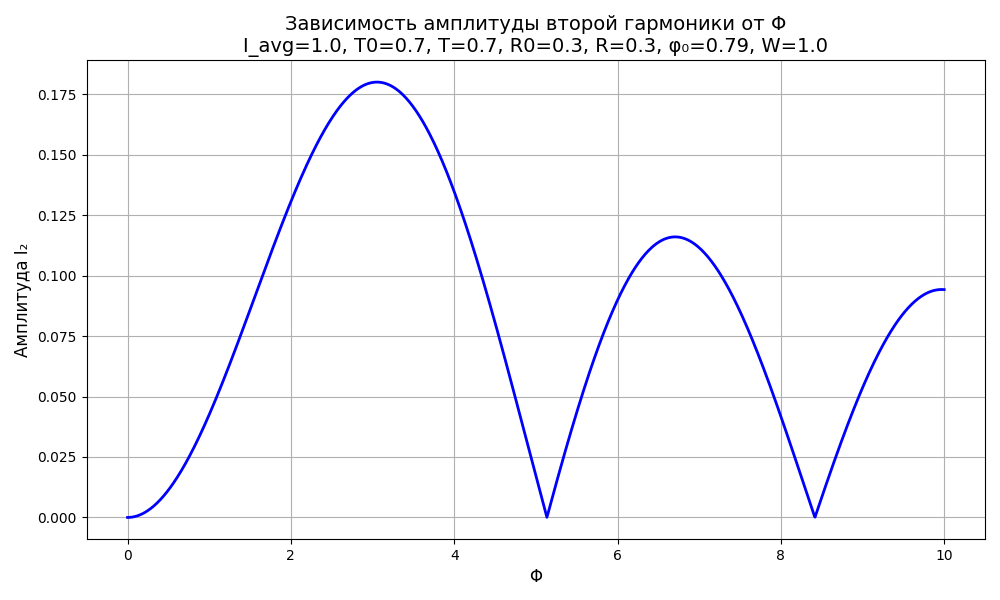
\includegraphics[width=0.5\textwidth]{../figures/second_harmonic_intensity_I1.0_T00.7_T0.7_R00.3_R0.3_phi0.79_W1.0.png}
  \caption{Вторая гармоника}
\end{figure}

\end{document}

